% IEEE BDDM 2026, Workshop 3 manuscript ("Workshop3 Pipeline" version), revision r1 of 2026-11-16.
% Rebuilt from BDDM2026_Workshop3_Pipeline_English_Manuscript.pdf because its original source was
% not available on this machine; see handoffs/D/2026-11-16_workshop3_latex_rebuild.md for every change.
% Red bracketed text marks items the author group must confirm before submission.
% Build: sh paper/latex-workshop3/build.sh   (or: pdflatex main, twice). No BibTeX run is needed.
% Self-contained: all four figures are drawn with TikZ/pgfplots from numbers in the formal run.
\documentclass[conference]{IEEEtran}
\IEEEoverridecommandlockouts

\usepackage[T1]{fontenc}
\usepackage{amsmath}
\usepackage{graphicx}
\usepackage{booktabs}
\usepackage{array}
\usepackage{multirow}
\usepackage{xcolor}
\usepackage{cite}
\usepackage[hidelinks]{hyperref}
\usepackage{url}
\usepackage{tikz}
\usepackage{pgfplots}
\pgfplotsset{compat=1.17}
\usepgfplotslibrary{groupplots}
\usetikzlibrary{shapes.multipart,arrows.meta,calc}

\definecolor{hospA}{RGB}{31,95,139}
\definecolor{hospB}{RGB}{181,84,26}
\definecolor{boxhdr}{RGB}{228,239,246}
\definecolor{boxframe}{RGB}{150,175,190}

\newcommand{\confirm}[1]{\textcolor{red}{[#1]}}
\newcommand{\pmean}{\bar{p}}

% Shared plot style.
\pgfplotsset{
  paper/.style={
    tick label style={font=\scriptsize},
    label style={font=\scriptsize},
    title style={font=\scriptsize\bfseries, at={(0,1)}, anchor=south west, inner sep=2pt},
    legend style={font=\scriptsize, draw=none, fill=none, inner sep=1pt},
    axis line style={black!60},
    tick style={black!60},
    ymajorgrids, grid style={black!10},
    axis x line*=bottom, axis y line*=left,
    tick align=outside,
  }
}

\begin{document}

\title{Imputation Disagreement for Selective Sepsis Prediction in Two Hospitals}

% Four authors, all at Beijing Jiaotong University; Jiang and Zhang are co-first authors (user decision, 2026-11-16).
\author{\IEEEauthorblockN{Yicheng Jiang\textsuperscript{*}, Shijie Zhang\textsuperscript{*}, Sirui Huang, Xufeng Yin}
\IEEEauthorblockA{Beijing Jiaotong University, China}
\thanks{\textsuperscript{*}These authors contributed equally to this work.}}

\maketitle

\begin{abstract}
We evaluated whether disagreement across imputed predictions helps identify which cases to defer in a retrospective sepsis prediction task. We used measurements through intensive care unit hour 12 to predict dataset-defined onset in hours (12, 24] in two hospitals from PhysioNet Challenge 2019. Of 24,095 eligible patients, 95 met the endpoint. Confidence, missingness and disagreement ranked the same singleton conformal predictions from a shared logistic regression model. At a matched target acceptance of 60\%, disagreement minus confidence selective risk was +0.109 percentage points internally (95\% paired bootstrap interval 0.000 to +0.328) and $-$0.036 externally ($-$0.108 to +0.036). External set coverage was 97.24\% overall and 0/38 among positives. Source-hospital cutoffs selected for a 60\% target yielded external acceptance of 89.05\% for confidence, 86.09\% for disagreement and 41.43\% for missingness. Disagreement showed no consistent risk reduction across splits. Six rule-selection errors prevented estimation of its added value conditional on confidence and missingness. Reporting class-specific coverage, paired patient decisions and realized acceptance exposed failures that aggregate coverage obscured.
\end{abstract}

\begin{IEEEkeywords}
selective prediction, conformal prediction, missing data, multiple imputation, sepsis
\end{IEEEkeywords}

\section{Introduction}

Early sepsis prediction depends on the measurements available when a decision is made~\cite{reyna2020}. Multiple imputation represents uncertainty about missing values with repeated draws~\cite{rubin1987,vanbuuren2011}. Even patients with similar mean predicted risks may differ in how much predictions vary across completions. Whether that variability helps identify errors at a given acceptance capacity is an empirical question.

Selective classification permits deferral, so comparisons must account for how many predictions each method accepts~\cite{geifman2017,traub2024}. The study addresses three questions. First, do the prediction sets retain the positive label for patients who experience the endpoint? Second, how much does imputation disagreement change selective risk and individual decisions at a shared acceptance quota? Third, what acceptance rates and false-negative counts result when source-hospital thresholds are applied directly to a held-out hospital? Fig.~\ref{fig:pipeline} shows the study design and separates the two acceptance rules.

The study is a reliability evaluation for a safety-critical prediction task, and it contributes three things. (i)~A matched protocol: confidence, missingness and disagreement rank the same singleton pool from the same predictor, imputation draws and conformal cutoff at the same acceptance count, so differences in selective risk are attributable to the ranking. (ii)~Patient-level failure reporting: class-specific coverage and paired dispositions of positive patients show that high aggregate coverage coexisted with exclusion of the true label for every positive patient. (iii)~Evidence on threshold transfer: cutoffs selected for a 60\% target in one hospital accepted between 41\% and 89\% of patients in the other. The main result for imputation disagreement is negative.

\section{Related Work}

Split conformal prediction constructs label sets with a marginal coverage guarantee under exchangeability~\cite{vovk2005,angelopoulos2023}. The guarantee concerns the true label's inclusion across the population. Coverage within each class and error among accepted predictions are distinct quantities. Weighted conformal prediction addresses covariate shift under additional assumptions~\cite{tibshirani2019}, and departures from exchangeability can degrade coverage~\cite{barber2023}. For rare outcomes, empirical external coverage and error counts by class are especially informative.

Prior work studies conformal prediction with imputed covariates~\cite{zaffran2023}, cost-aware clinical deferral~\cite{kwon2026}, and conformal selection of individual imputed values~\cite{he2026}. Li et al. used separate target-cohort partitions for prevalence correction, calibration and evaluation in an audit of conformal triage~\cite{li2026}. Our comparison uses patient-level predictions and holds the predictor, imputation draws and singleton pool fixed. The external site supplies evaluation data, with all calibration and rule selection performed at the source site.

% ---------------------------------------------------------------- Fig. 1
\begin{figure*}[t]
\centering
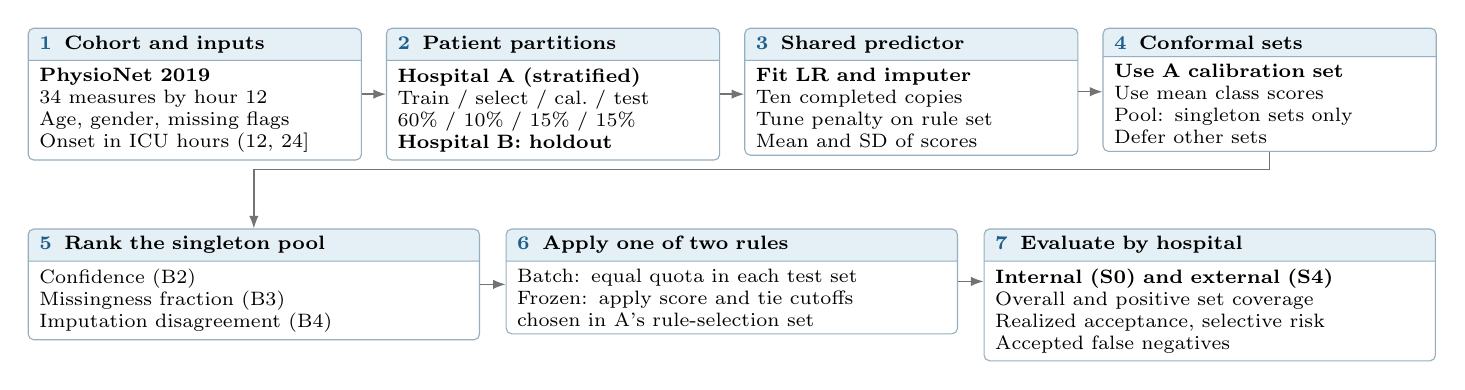
\begin{tikzpicture}[
  pbox/.style={rectangle split, rectangle split parts=2, draw=boxframe, rounded corners=2pt,
               rectangle split part fill={boxhdr,white}, align=left, inner xsep=4pt, inner ysep=2.5pt,
               font=\scriptsize, anchor=north west},
  flow/.style={-{Latex[length=1.6mm,width=1.2mm]}, draw=black!55, line width=0.5pt}]
\newcommand{\hd}[2]{\textbf{\textcolor{hospA}{#1}\enspace #2}}
% Row 1: four boxes, 4.27 cm text width, 0.28 cm gaps.
\node[pbox, text width=3.95cm] (b1) at (0,0)
  {\hd{1}{Cohort and inputs}
   \nodepart{two}\textbf{PhysioNet 2019}\\ 34 measures by hour 12\\ Age, gender, missing flags\\ Onset in ICU hours (12, 24]};
\node[pbox, text width=3.95cm] (b2) at (4.55,0)
  {\hd{2}{Patient partitions}
   \nodepart{two}\textbf{Hospital A (stratified)}\\ Train / select / cal.\ / test\\ 60\% / 10\% / 15\% / 15\%\\ \textbf{Hospital B: holdout}};
\node[pbox, text width=3.95cm] (b3) at (9.10,0)
  {\hd{3}{Shared predictor}
   \nodepart{two}\textbf{Fit LR and imputer}\\ Ten completed copies\\ Tune penalty on rule set\\ Mean and SD of scores};
\node[pbox, text width=3.95cm] (b4) at (13.65,0)
  {\hd{4}{Conformal sets}
   \nodepart{two}\textbf{Use A calibration set}\\ Use mean class scores\\ Pool: singleton sets only\\ Defer other sets};
% Row 2: three boxes.
\node[pbox, text width=5.45cm] (b5) at (0,-2.55)
  {\hd{5}{Rank the singleton pool}
   \nodepart{two}Confidence (B2)\\ Missingness fraction (B3)\\ Imputation disagreement (B4)};
\node[pbox, text width=5.45cm] (b6) at (6.07,-2.55)
  {\hd{6}{Apply one of two rules}
   \nodepart{two}Batch: equal quota in each test set\\ Frozen: apply score and tie cutoffs\\ chosen in A's rule-selection set};
\node[pbox, text width=5.45cm] (b7) at (12.14,-2.55)
  {\hd{7}{Evaluate by hospital}
   \nodepart{two}\textbf{Internal (S0) and external (S4)}\\ Overall and positive set coverage\\ Realized acceptance, selective risk\\ Accepted false negatives};
\draw[flow] (b1.east) -- (b1.east -| b2.west);
\draw[flow] (b2.east) -- (b2.east -| b3.west);
\draw[flow] (b3.east) -- (b3.east -| b4.west);
\draw[flow] (b4.south) -- ++(0,-0.22) -| (b5.north);
\draw[flow] (b5.east) -- (b5.east -| b6.west);
\draw[flow] (b6.east) -- (b6.east -| b7.west);
\end{tikzpicture}
\caption{Study pipeline for the primary logistic regression (LR) analysis. ICU denotes intensive care unit. The mean score and the source calibration cutoff at $\alpha = 0.10$ determine the prediction set. The standard deviation (SD) across ten imputed predictions is the disagreement score. Batch allocation uses the same singleton pool and quota for all rankings within each test set. Frozen rules apply source cutoffs without adjusting test acceptance.}
\label{fig:pipeline}
\end{figure*}

\section{Methods}

\subsection{Cohort, Outcome and Partitions}

We used the two public training sets of the PhysioNet/Computing in Cardiology Challenge 2019, version 1.0.0~\cite{reyna2019data,pollard2026}. The source derived onset labels from criteria based on Sepsis-3~\cite{reyna2020,singer2016}. We required records to start at intensive care unit (ICU) hour 1 and contain every hour through hour 24. We checked hour indices and binary, monotone labels. For an observed zero-to-one transition at hour $t$, the onset proxy was $t+6$ hours. We excluded records already positive at the first observation and patients whose recovered onset was at or before hour 12. Eligible records with recovered onset in $(12, 24]$ were positive. Eligible records without a positive label or with recovered onset after hour 24 were window negatives.

Each of 34 physiological and laboratory variables was represented by its last observed value through hour 12. Unobserved values remained missing. We also used age, the dataset's recorded gender variable and a missingness indicator for each of the 36 inputs. We stratified Hospital A by outcome into training, rule selection, calibration and internal test sets in proportions of approximately 60\%, 10\%, 15\% and 15\%. Hospital B was held out in full. Seed 2026 defined the primary split. Seeds 2027--2030 changed the split in Hospital A and reused Hospital B.

\subsection{Imputation and Prediction}

We fitted a ten-round Bayesian ridge chained-equation imputer on training covariates. For each completed input, we initialized physiological and laboratory variables with training medians, sampled from the fitted conditional Gaussian predictions at missing entries and clipped the final draws to training-observed ranges. Observed entries were preserved. Age and recorded gender used the training median and mode, respectively. Variables missing throughout training contributed only their missingness indicators.

One standardized, $L_2$-regularized logistic regression (LR) classifier was fitted to $M = 10$ completed copies of the training patients, weighting each copy by $1/M$. The regularization parameter $C \in \{0.1, 1, 10\}$ maximized average precision on the rule-selection set, with ties favoring the smaller value. Let $p_{im}$ be patient $i$'s predicted positive probability on draw $m$. We used the mean $\pmean_i = M^{-1}\sum_{m=1}^{M} p_{im}$ and the sample standard deviation
\begin{equation}
d_i = \sqrt{\frac{1}{M-1}\sum_{m=1}^{M}\left(p_{im}-\pmean_i\right)^2}.
\label{eq:disagreement}
\end{equation}

\subsection{Conformal Sets and Selection Rules}

Let $\pmean_i(1) = \pmean_i$ and $\pmean_i(0) = 1-\pmean_i$. We computed the calibration scores $1-\pmean_i(y_i)$, where $y_i$ is the true label. The cutoff $q$ is the $k$th smallest score, where $k = \lceil (n_{\mathrm{cal}}+1)(1-\alpha) \rceil$ and $\alpha = 0.10$. If $k > n_{\mathrm{cal}}$, $q$ is infinite. The prediction set contains labels $y$ with $1-\pmean_i(y) \le q$. Empty and two-label sets are deferred. A singleton can be accepted with its sole label.

With $N$ test patients and $N_{\mathrm{sing}}$ singletons, batch allocation accepts the first $K = \min\{\lfloor cN \rfloor, N_{\mathrm{sing}}\}$ ranked singletons for target $c \in \{0.40, 0.60, 0.80\}$. Confidence (B2) ranks by increasing $\min(\pmean_i, 1-\pmean_i)$, missingness (B3) by the missing fraction of the 34 physiological and laboratory variables, and disagreement (B4) by increasing $d_i$. A fixed patient-identifier hash resolves ties. The all-singleton baselines use either median imputation with a separately fitted classifier of the same type and separate calibration (B0) or the multiple-imputation mean score (B1).

The prespecified error-risk models use standardized confidence and missingness predictors (B5) and add $d_i$ (B6). Both use $L_2$-regularized LR with $C = 1$. Fitting uses all rule-selection patients and targets base prediction error at threshold 0.5. It requires at least 20 errors and 20 correct predictions. For frozen-threshold evaluation, we used the calibrated singleton pool in the rule-selection set to choose each score cutoff and tie rule at the target quota. We applied those cutoffs to test singletons without recalibration or a test quota.

% ---------------------------------------------------------------- Table I
\begin{table}[t]
\caption{Primary Partition Sizes and Endpoint Counts}
\label{tab:partitions}
\centering
\footnotesize
\begin{tabular}{lrrr}
\toprule
Role & Patients & Events & Event rate (\%)\\
\midrule
Train & 6,104 & 34 & 0.557\\
Selection & 1,018 & 6 & 0.589\\
Calibration & 1,527 & 9 & 0.589\\
Test & 1,525 & 8 & 0.525\\
External & 13,921 & 38 & 0.273\\
\bottomrule
\end{tabular}
\end{table}

% ---------------------------------------------------------------- Fig. 2
\begin{figure}[t]
\centering
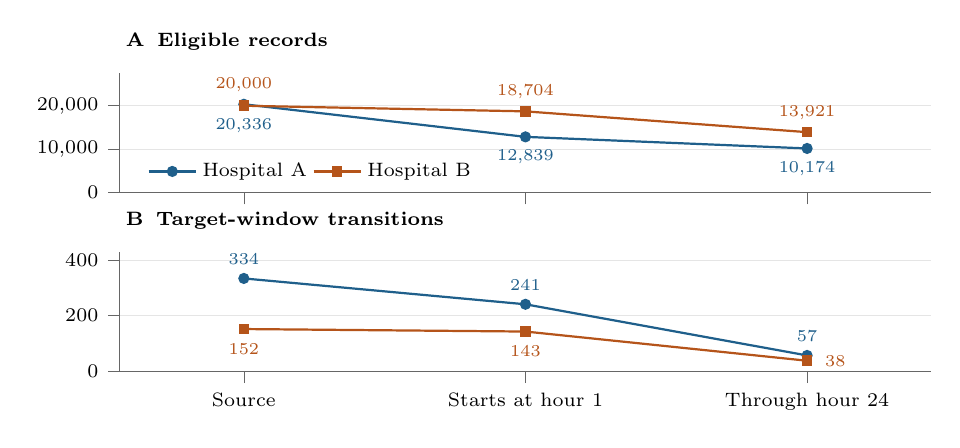
\begin{tikzpicture}
\begin{groupplot}[paper,
  group style={group size=1 by 2, vertical sep=0.75cm},
  width=0.98\columnwidth, height=3.1cm,
  symbolic x coords={Source,Starts at hour 1,Through hour 24},
  xtick=data, enlarge x limits=0.22, scaled y ticks=false]
\nextgroupplot[title={A\enspace Eligible records}, ymin=0, ymax=27500,
  ytick={0,10000,20000}, yticklabels={0,{10,000},{20,000}}, xticklabels={},
  legend pos=south west, legend columns=2]
\addplot[hospA, thick, mark=*, mark size=1.6pt] coordinates
  {(Source,20336) (Starts at hour 1,12839) (Through hour 24,10174)};
\addplot[hospB, thick, mark=square*, mark size=1.5pt] coordinates
  {(Source,20000) (Starts at hour 1,18704) (Through hour 24,13921)};
\legend{Hospital A, Hospital B}
\node[font=\fontsize{6}{7}\selectfont, hospB, anchor=south] at (axis cs:Source,20900) {20,000};
\node[font=\fontsize{6}{7}\selectfont, hospA, anchor=north] at (axis cs:Source,19300) {20,336};
\node[font=\fontsize{6}{7}\selectfont, hospB, anchor=south] at (axis cs:Starts at hour 1,19400) {18,704};
\node[font=\fontsize{6}{7}\selectfont, hospA, anchor=north] at (axis cs:Starts at hour 1,12000) {12,839};
\node[font=\fontsize{6}{7}\selectfont, hospB, anchor=south] at (axis cs:Through hour 24,14600) {13,921};
\node[font=\fontsize{6}{7}\selectfont, hospA, anchor=north] at (axis cs:Through hour 24,9400) {10,174};
\nextgroupplot[title={B\enspace Target-window transitions}, ymin=0, ymax=430, ytick={0,200,400}]
\addplot[hospA, thick, mark=*, mark size=1.6pt] coordinates
  {(Source,334) (Starts at hour 1,241) (Through hour 24,57)};
\addplot[hospB, thick, mark=square*, mark size=1.5pt] coordinates
  {(Source,152) (Starts at hour 1,143) (Through hour 24,38)};
\node[font=\fontsize{6}{7}\selectfont, hospA, anchor=south] at (axis cs:Source,350) {334};
\node[font=\fontsize{6}{7}\selectfont, hospB, anchor=north] at (axis cs:Source,135) {152};
\node[font=\fontsize{6}{7}\selectfont, hospA, anchor=south] at (axis cs:Starts at hour 1,257) {241};
\node[font=\fontsize{6}{7}\selectfont, hospB, anchor=north] at (axis cs:Starts at hour 1,126) {143};
\node[font=\fontsize{6}{7}\selectfont, hospA, anchor=south] at (axis cs:Through hour 24,73) {57};
\node[font=\fontsize{6}{7}\selectfont, hospB, anchor=west, xshift=3pt] at (axis cs:Through hour 24,38) {38};
\end{groupplot}
\end{tikzpicture}
\caption{Sequential cohort eligibility and target-window transitions. Panel A counts records at each step. Panel B counts label-derived onset proxies in the target window.}
\label{fig:attrition}
\end{figure}

\subsection{Metrics, Uncertainty and Sensitivity}

Selective risk divides incorrect accepted predictions by all accepted predictions. The accepted false-negative fraction among positives divides accepted negative predictions for true positives by all positives. Realized acceptance divides the accepted count by the test cohort size. Set coverage counts how often the true label is in the original prediction set before selection. We report area under the receiver operating characteristic curve (AUROC) and average precision (AP) for the underlying scores, with 95\% intervals for AUROC from 1,000 bootstrap resamples.

The primary comparison was B4 minus B2 selective risk at a 60\% batch target with the primary LR model and the first imputation batch. S0 denotes internal natural missingness and S4 denotes external natural missingness. We report paired 95\% percentile intervals from 1,000 patient bootstrap resamples, recomputing quotas and rankings for batch allocation and resampling fixed decisions for frozen thresholds. The fitted predictor and conformal cutoff stayed fixed. Positive-class coverage intervals are two-sided exact binomial intervals conditional on the fitted rule. In a post hoc analysis, we replayed the primary comparison from frozen inputs to cross-tabulate the dispositions of positive patients under B2 and B4. Replayed cutoffs and aggregate metrics agreed with the formal run.

S1 and S2 independently mask observed physiological or laboratory inputs at test time with probabilities 0.10 and 0.30. S3 masks the laboratory block (columns 9--34). All rankings use the same masks, and training and calibration remain at natural missingness. Sensitivity checks use a 300-tree random forest in S0/S2, $M = 5$ and 20 in S0, and $\alpha = 0.05$ in S0/S2. Five test-time imputation batches in S0 permit pairwise comparisons of the three possible decisions: accept negative, accept positive or defer.

A post hoc reference draws $K$ singletons uniformly without replacement from the observed pool. The false-negative count follows a hypergeometric distribution with population size $N_{\mathrm{sing}}$, number of false negatives in the pool $F$, and draw size $K$. Its mean is $KF/N_{\mathrm{sing}}$. We report the 2.5th and 97.5th percentiles as a descriptive allocation range conditional on the observed pool.

% ---------------------------------------------------------------- Table II
\begin{table*}[t]
\caption{Matched Batch Capacity and Frozen-Threshold Transfer at a 60\% Target in the Primary Split. FN Counts Positive Patients Accepted as Negative.}
\label{tab:transfer}
\centering
\footnotesize
\begin{tabular}{llrrrr}
\toprule
 & & \multicolumn{2}{c}{Matched batch} & \multicolumn{2}{c}{Frozen threshold}\\
\cmidrule(lr){3-4}\cmidrule(lr){5-6}
Test set & Ranking & Accepted (\%) & FN / positives & Accepted (\%) & FN / positives\\
\midrule
Internal & Confidence (B2) & 915 (60.00) & 1/8 & 919 (60.26) & 1/8\\
 & Missingness (B3) & 915 (60.00) & 2/8 & 915 (60.00) & 2/8\\
 & Disagreement (B4) & 915 (60.00) & 2/8 & 928 (60.85) & 2/8\\
\addlinespace
External & Confidence (B2) & 8,352 (60.00) & 24/38 & 12,396 (89.05) & 33/38\\
 & Missingness (B3) & 8,352 (60.00) & 24/38 & 5,768 (41.43) & 19/38\\
 & Disagreement (B4) & 8,352 (60.00) & 21/38 & 11,984 (86.09) & 34/38\\
\bottomrule
\end{tabular}
\end{table*}

% ---------------------------------------------------------------- Fig. 3
\begin{figure*}[t]
\centering
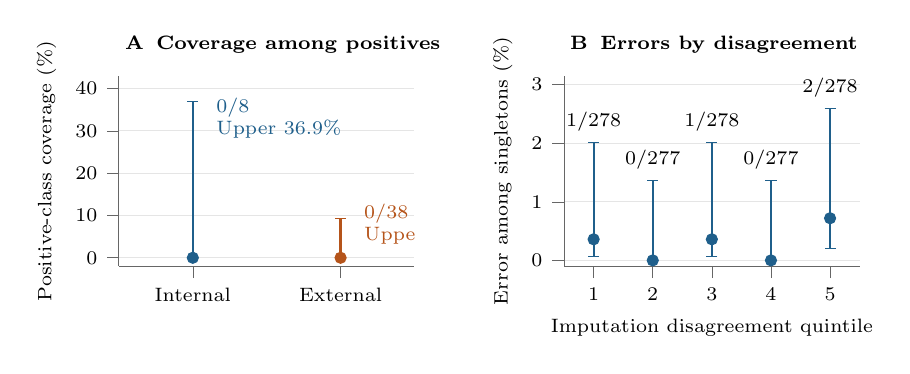
\begin{tikzpicture}
\begin{groupplot}[paper,
  group style={group size=2 by 1, horizontal sep=1.9cm},
  width=0.44\textwidth, height=4.0cm]
\nextgroupplot[title={A\enspace Coverage among positives},
  symbolic x coords={Internal,External}, xtick={Internal,External}, enlarge x limits=0.5,
  ymin=-2, ymax=43, ytick={0,10,20,30,40}, ylabel={Positive-class coverage (\%)}]
\addplot[hospA, only marks, mark=*, mark size=2pt,
  error bars/.cd, y dir=plus, y explicit, error bar style={thick}]
  coordinates {(Internal,0) +- (0,36.9)};
\addplot[hospB, only marks, mark=*, mark size=2pt,
  error bars/.cd, y dir=plus, y explicit, error bar style={thick}]
  coordinates {(External,0) +- (0,9.25)};
\node[font=\scriptsize, hospA, anchor=west, align=left, xshift=5pt] at (axis cs:Internal,33) {0/8\\ Upper 36.9\%};
\node[font=\scriptsize, hospB, anchor=west, align=left, xshift=5pt] at (axis cs:External,8) {0/38\\ Upper 9.3\%};
\nextgroupplot[title={B\enspace Errors by disagreement},
  xmin=0.5, xmax=5.5, xtick={1,2,3,4,5}, ymin=-0.1, ymax=3.15, ytick={0,1,2,3},
  xlabel={Imputation disagreement quintile}, ylabel={Error among singletons (\%)}]
% Wilson 95% intervals for 1/278, 0/277, 1/278, 0/277 and 2/278.
\addplot[hospA, only marks, mark=*, mark size=2pt,
  error bars/.cd, y dir=both, y explicit, error bar style={thick}]
  coordinates {
    (1,0.3597) += (0,1.6494) -= (0,0.2962)
    (2,0.0000) += (0,1.3679) -= (0,0.0000)
    (3,0.3597) += (0,1.6494) -= (0,0.2962)
    (4,0.0000) += (0,1.3679) -= (0,0.0000)
    (5,0.7194) += (0,1.8654) -= (0,0.5220)};
\node[font=\scriptsize, anchor=south] at (axis cs:1,2.03) {1/278};
\node[font=\scriptsize, anchor=south] at (axis cs:2,1.39) {0/277};
\node[font=\scriptsize, anchor=south] at (axis cs:3,2.03) {1/278};
\node[font=\scriptsize, anchor=south] at (axis cs:4,1.39) {0/277};
\node[font=\scriptsize, anchor=south] at (axis cs:5,2.61) {2/278};
\end{groupplot}
\end{tikzpicture}
\caption{Positive-class coverage and errors in the primary split. Panel A gives exact 95\% intervals for class coverage. Panel B gives error counts and Wilson 95\% intervals by disagreement quintile among internal singleton predictions.}
\label{fig:coverage}
\end{figure*}

\section{Results}

\subsection{Cohort and Event Attrition}

Of 40,336 source records, 24,095 met the eligibility rules. Hospital A contributed 10,174 patients and 57 events, and Hospital B contributed 13,921 patients and 38 events. The primary Hospital A split contained 34 training, 6 rule-selection, 9 calibration and 8 test positives (Table~\ref{tab:partitions}).

An exploratory raw-record audit identified 486 transitions whose recovered onset fell in the target window. The start-hour rule removed 102 of these transitions. The subsequent follow-up rule removed 289, including one whose recovered onset fell beyond the available record. The remaining 95 constituted 19.5\% of the 486 transitions (Fig.~\ref{fig:attrition}). These are label-based counts. The audit reproduced all eligible labels and feature values in the frozen inputs.

\subsection{Prediction-Set Coverage and Discrimination}

The selected LR had $C = 0.1$. Internally, AUROC was 0.793 (95\% interval $[0.579, 0.947]$) and AP was 0.0292 at a prevalence of 0.525\%. Externally, AUROC was 0.502 ($[0.407, 0.596]$) and AP was 0.00293 at a prevalence of 0.273\%. The pooled cutoff $q \approx 0.01098$ required a positive score of at least $1-q \approx 0.98902$ for label 1 to enter a set. Overall coverage was 1,384/1,525 (90.75\%) internally and 13,537/13,921 (97.24\%) externally. Positive-class coverage was 0/8 and 0/38, with exact 95\% intervals of 0--36.9\% and 0--9.25\%, respectively (Fig.~\ref{fig:coverage}a). The primary singleton pools contained 1,388 patients internally and 13,575 externally, all with negative predictions. The pools included four internal positives and all 38 external positives. The other four internal positives had empty sets. Accepting every singleton (B1) would therefore accept 91.02\% of internal patients and 97.51\% of external patients, including all positives in the respective pools. The median-imputation baseline (B0) behaved similarly: its singleton pools held 1,380 internal and 13,143 external patients (90.49\% and 94.41\%), all with negative predictions, and included 4 of 8 and 37 of 38 positives.

\subsection{Matched Capacity and Threshold Transfer}

At the 60\% target, each ranking accepted 915 internal patients and 8,352 external patients (Table~\ref{tab:transfer}). Disagreement versus confidence yielded one more accepted error internally and three fewer externally. The selective-risk difference was +0.109 percentage points internally (95\% paired interval $[0.000, +0.328]$) and $-$0.036 externally ($[-0.108, +0.036]$). Missingness matched disagreement's error count internally and confidence's externally. At the other two prespecified targets, disagreement and confidence accepted 1 and 1 positives as negative internally at 40\% and 2 and 3 at 80\%; externally the counts were 18 and 15 at 40\% and 30 and 29 at 80\%, so the direction of the difference varied with the quota.

Uniform ranking at the same quota would accept 2.64 false negatives on average internally (central 95\% range 1--4) and 23.38 externally (17--29). The observed false-negative counts for all three rankings fell within these ranges in both cohorts.

Under matched external capacity, both rankings accepted 18 positive patients as negative and both deferred 11. Switching from confidence to disagreement deferred six previously accepted positives and accepted three previously deferred positives as negative. Internally, both rankings accepted one positive as negative and both deferred six. Switching to disagreement accepted one additional positive as negative.

Frozen thresholds produced internal acceptance near the target. External acceptance rose to 89.05\% for confidence and 86.09\% for disagreement, with accepted false negatives increasing from 24 to 33 and from 21 to 34, respectively. The external frozen-threshold risk difference was +0.017 percentage points ($[-0.017, +0.052]$), at the two different realized acceptance rates. The missingness cutoff accepted 41.43\% externally, including 19/38 positives as negatives. Across all five splits, external acceptance was above target for confidence (79.48--89.54\%) and disagreement (72.33--86.29\%) and below target for missingness (38.68--41.43\%).

% ---------------------------------------------------------------- Fig. 4
\begin{figure}[t]
\centering
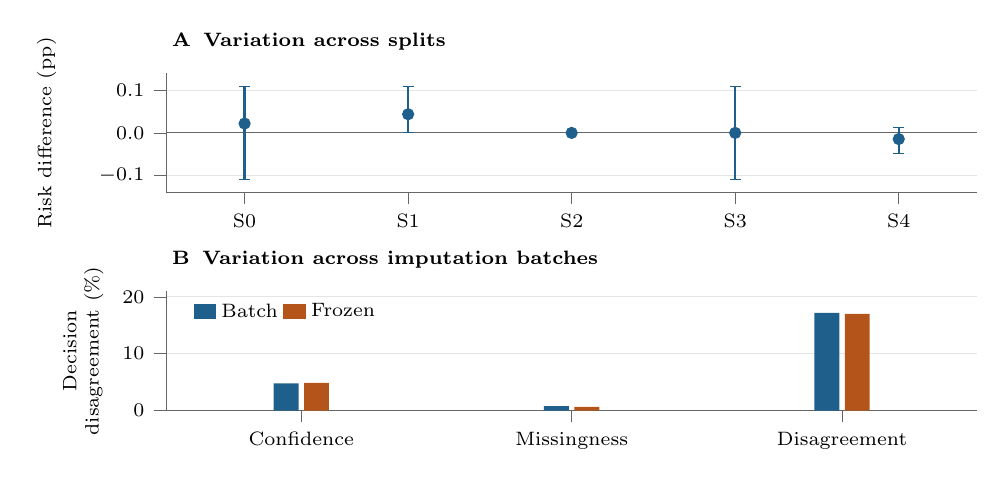
\begin{tikzpicture}
\begin{groupplot}[paper,
  group style={group size=1 by 2, vertical sep=1.25cm},
  width=0.98\columnwidth, height=3.1cm]
\nextgroupplot[title={A\enspace Variation across splits},
  symbolic x coords={S0,S1,S2,S3,S4}, xtick=data, enlarge x limits=0.12,
  ymin=-0.14, ymax=0.14, ytick={-0.1,0,0.1}, yticklabels={$-$0.1,0.0,0.1},
  ylabel={Risk difference (pp)}, extra y ticks={0}, extra y tick labels={},
  extra y tick style={grid style={black!60}}]
% Mean and observed range of B4 minus B2 over seeds 2026-2030 (60% batch target).
\addplot[hospA, only marks, mark=*, mark size=2pt,
  error bars/.cd, y dir=both, y explicit, error bar style={thick}]
  coordinates {
    (S0,0.0219)  += (0,0.0874) -= (0,0.1312)
    (S1,0.0437)  += (0,0.0656) -= (0,0.0437)
    (S2,0.0000)  += (0,0.0000) -= (0,0.0000)
    (S3,0.0000)  += (0,0.1093) -= (0,0.1093)
    (S4,-0.0144) += (0,0.0264) -= (0,0.0335)};
\nextgroupplot[title={B\enspace Variation across imputation batches},
  ybar, bar width=9pt, symbolic x coords={Confidence,Missingness,Disagreement},
  xtick=data, enlarge x limits=0.25, ymin=0, ymax=21, ytick={0,10,20},
  ylabel={Decision\\disagreement (\%)}, ylabel style={align=center}, legend pos=north west, legend columns=2,
  legend image code/.code={\draw[#1,draw=none] (0cm,-0.08cm) rectangle (0.28cm,0.1cm);}]
\addplot[fill=hospA, draw=none] coordinates {(Confidence,4.79) (Missingness,0.79) (Disagreement,17.18)};
\addplot[fill=hospB, draw=none] coordinates {(Confidence,4.90) (Missingness,0.66) (Disagreement,16.98)};
\legend{Batch, Frozen}
\end{groupplot}
\end{tikzpicture}
\caption{Sensitivity across splits and imputation draws at the 60\% target. Panel A shows means and observed ranges across five splits. Panel B shows mean pairwise decision disagreement across five imputation batches in the primary internal test.}
\label{fig:sensitivity}
\end{figure}

\subsection{Stability and Sensitivity}

At the primary batch capacity, B4 minus B2 changed sign across splits in S0 and S4, and the observed difference was zero in S2 for all five splits (Fig.~\ref{fig:sensitivity}a). Across the ten pairs of S0 imputation batches in the primary split, mean decision disagreement was 17.18\% for B4, 4.79\% for B2 and 0.79\% for B3 under batch allocation. The corresponding frozen-rule values were 16.98\%, 4.90\% and 0.66\% (Fig.~\ref{fig:sensitivity}b). The random forest yielded a B4 minus B2 risk difference of +0.219 percentage points in S0 and S2 at the primary batch capacity, with both intervals including zero. Changing the draw count or $\alpha$ yielded differences at or above zero in the tested internal settings.

The primary rule-selection set had six errors and 1,012 correct predictions. The error count did not meet the 20-error minimum for B5/B6, so the incremental contrast conditional on confidence and missingness was unestimable. The internal singleton pool contained only four errors. Their sparse distribution across disagreement quintiles limits inference about the ranking signal (Fig.~\ref{fig:coverage}b).

\section{Discussion}

At matched capacity, the external reduction of three false negatives with disagreement combined discordant decisions in both directions. The interval for the external risk difference spanned zero. All three observed false-negative counts also fell within the post hoc random-allocation range, including the counts for confidence and missingness. This reference describes how variable a quota-sized draw would be in each observed pool. It provides neither an equivalence margin nor a formal test of ranking quality. With an external AUROC of 0.502, the external comparison contrasts orderings of scores that barely separate outcomes; we read it as evidence about failure under transfer, not about the quality of the ranking signals.

The frozen-rule comparison measures performance at the acceptance rate each cutoff produces. Confidence and disagreement accepted more than the 60\% target externally and missed more positives than under matched allocation. The missingness rule accepted fewer cases and missed 19 of the 38 positives. Its lower missed count came with lower realized acceptance. The equal-capacity comparison isolates differences between rankings at the same acceptance workload.

The 97.24\% external coverage was driven by negatives. In the primary setting, every positive patient's score fell short of the threshold needed to include label 1. The study cannot isolate the contributions of score quality, site differences and pooled calibration to that result. Label-conditional calibration targets coverage within each outcome class under within-class exchangeability~\cite{sadinle2019}. Ajit applies a related stratified approach to modality-availability groups~\cite{ajit2026}. With nine positive calibration patients and $\alpha = 0.10$, the label-conditional positive cutoff would be the largest of nine scores. The resulting coverage and singleton capacity would require separate evaluation. The primary internal test had only eight positives, so changing the disposition of one positive moves any rate with that denominator by 12.5 percentage points.

The eligibility requirement for records through hour 24 constrains the population and removes many observable label transitions. The onset proxy depends on the challenge labels and their offset. Relaxing the follow-up rule would require a definition of observable negative outcomes for patients whose records end before hour 24. One hospital supplied the external data, and the five splits reuse those patients. The bootstrap describes test-cohort variation conditional on fitted rules, with limited resolution when errors are sparse. The test masks are controlled perturbations, and repeated imputations reflect variability under the fitted procedure. The larger batch-to-batch variation for disagreement therefore describes this pipeline. Establishing added predictive value or clinical workflow benefit requires additional events and a separate evaluation.

\section{Conclusion}

In this retrospective two-hospital cohort, imputation disagreement showed no consistent selective-risk advantage over confidence at matched capacity. High external set coverage coexisted with zero positive-class coverage, and the three source thresholds produced external acceptance between 41.43\% and 89.05\%. Reporting class-specific coverage, the composition of the singleton pool and paired decisions alongside realized acceptance makes these outcomes visible.

\section*{Data and Code Availability}

This secondary analysis used public, de-identified PhysioNet data~\cite{reyna2020,reyna2019data}; no new patient data were collected, and we do not redistribute patient-level records. Analysis code, aggregate results and replay scripts are available at \url{https://github.com/MarcoJIANG5203/BDDM-10}.

\section*{Acknowledgment}

Generative AI tools (OpenAI Codex and Anthropic Claude) assisted with English drafting and revision throughout the manuscript, numerical and reference checks, and preparation of the pipeline and aggregate figures. The authors reviewed all content and are responsible for the manuscript and its interpretation.

\begin{thebibliography}{18}
\providecommand{\doi}[1]{doi: \nolinkurl{#1}}

\bibitem{reyna2020}
M.~A. Reyna \emph{et al.}, ``Early prediction of sepsis from clinical data: The PhysioNet/Computing in Cardiology Challenge 2019,'' \emph{Crit. Care Med.}, vol.~48, no.~2, pp. 210--217, 2020, \doi{10.1097/CCM.0000000000004145}.

\bibitem{rubin1987}
D.~B. Rubin, \emph{Multiple Imputation for Nonresponse in Surveys}. New York, NY, USA: Wiley, 1987, \doi{10.1002/9780470316696}.

\bibitem{vanbuuren2011}
S.~van Buuren and K.~Groothuis-Oudshoorn, ``mice: Multivariate imputation by chained equations in R,'' \emph{J. Stat. Softw.}, vol.~45, no.~3, pp. 1--67, 2011, \doi{10.18637/jss.v045.i03}.

\bibitem{geifman2017}
Y.~Geifman and R.~El-Yaniv, ``Selective classification for deep neural networks,'' in \emph{Adv. Neural Inf. Process. Syst.}, vol.~30, 2017. [Online]. Available: \url{https://papers.neurips.cc/paper/7073-selective-classification-for-deep-neural-networks}

\bibitem{traub2024}
J.~Traub \emph{et al.}, ``Overcoming common flaws in the evaluation of selective classification systems,'' in \emph{Adv. Neural Inf. Process. Syst.}, vol.~37, 2024, pp. 2323--2347, \doi{10.52202/079017-0076}.

\bibitem{vovk2005}
V.~Vovk, A.~Gammerman, and G.~Shafer, \emph{Algorithmic Learning in a Random World}. New York, NY, USA: Springer, 2005, \doi{10.1007/b106715}.

\bibitem{angelopoulos2023}
A.~N. Angelopoulos and S.~Bates, ``Conformal prediction: A gentle introduction,'' \emph{Found. Trends Mach. Learn.}, vol.~16, no.~4, pp. 494--591, 2023, \doi{10.1561/2200000101}.

\bibitem{tibshirani2019}
R.~J. Tibshirani, R.~F. Barber, E.~J. Cand\`es, and A.~Ramdas, ``Conformal prediction under covariate shift,'' in \emph{Adv. Neural Inf. Process. Syst.}, vol.~32, 2019. [Online]. Available: \url{https://proceedings.neurips.cc/paper/2019/hash/8fb21ee7a2207526da55a679f0332de2-Abstract.html}

\bibitem{barber2023}
R.~F. Barber, E.~J. Cand\`es, A.~Ramdas, and R.~J. Tibshirani, ``Conformal prediction beyond exchangeability,'' \emph{Ann. Statist.}, vol.~51, no.~2, pp. 816--845, 2023, \doi{10.1214/23-AOS2276}.

\bibitem{zaffran2023}
M.~Zaffran, A.~Dieuleveut, J.~Josse, and Y.~Romano, ``Conformal prediction with missing values,'' in \emph{Proc. 40th Int. Conf. Mach. Learn.}, PMLR, vol.~202, 2023, pp. 40578--40604.

\bibitem{kwon2026}
H.~Kwon and D.-J. Kim, ``Conformal selective prediction with cost aware deferral for safe clinical triage under distribution shift,'' \emph{Sci. Rep.}, vol.~16, Art. no. 10016, 2026, \doi{10.1038/s41598-026-40637-w}.

\bibitem{he2026}
X.~He, M.~Ai, J.~Wang, C.~B. Cook, and J.~He, ``SafeImpute: Reliable clinical data imputation via conformal selection,'' in \emph{Proc. 32nd ACM SIGKDD Conf. Knowl. Discov. Data Min.}, vol.~2, 2026, pp. 1626--1637, \doi{10.1145/3770855.3817967}.

\bibitem{li2026}
C.~Li \emph{et al.}, ``A deployment audit of release-side risk in conformal triage under prevalence shift,'' in \emph{Proc. 15th Symp. Conformal Probab. Predict. Appl.}, PMLR, vol.~329, 2026, pp. 793--812.

\bibitem{reyna2019data}
M.~Reyna \emph{et al.}, ``Early prediction of sepsis from clinical data: The PhysioNet/Computing in Cardiology Challenge 2019,'' PhysioNet, version 1.0.0, 2019, \doi{10.13026/v64v-d857}.

\bibitem{pollard2026}
T.~Pollard \emph{et al.}, ``PhysioNet as a global platform for biomedical research,'' \emph{Nature Health}, vol.~1, no.~8, pp. 792--795, 2026, \doi{10.1038/s44360-026-00096-z}.

\bibitem{singer2016}
M.~Singer \emph{et al.}, ``The Third International Consensus Definitions for Sepsis and Septic Shock (Sepsis-3),'' \emph{JAMA}, vol.~315, no.~8, pp. 801--810, 2016, \doi{10.1001/jama.2016.0287}.

\bibitem{sadinle2019}
M.~Sadinle, J.~Lei, and L.~Wasserman, ``Least ambiguous set-valued classifiers with bounded error levels,'' \emph{J. Amer. Statist. Assoc.}, vol.~114, no.~525, pp. 223--234, 2019, \doi{10.1080/01621459.2017.1395341}.

\bibitem{ajit2026}
A.~Ajit, ``Guarantees that survive a missing scan: Modality-conditional conformal prediction for multimodal medical diagnosis,'' in \emph{Proc. 17th Int. Workshop Mach. Learn. Med. Imag.}, MICCAI Satellite Events, 2026. [Online]. Available: \url{https://papers.miccai.org/miccai-2026-sat/MLMI_024.html}

\end{thebibliography}

\end{document}
